\chapter{Zweite Methode} \label{cha:ZweiteMethode}

In diesem Kapitel wird die Realisierung des zweiten Verfahrens eingegangen werden. Zuerst wird die allgemeine Struktur dieser Methode beschrieben. Dadurch können die Struktur und Arbeitsprinzip der gesamten Methode eine grobe verstehen. Anschießen geben die Bildverarbeitungen im Detail. Es besteht aus verschiedene Teile wie als folgend: Binarisierung Behandelung, Morphologie Operation und Canny Kannten Detektion. In diesem Abschnitt wird es  erläutert, wie diese Operationen funktioniert und was die Sinne dieser Behandelungen sind. Schließlich wird eine Linie Extrahieren Methode Hough Transformation detailliert vorstellen. Zur Implementierung dieses Verfahrens wird Matlab unter der Lizenz TU Dortmund verwendet. Außerdem diese Methode wird auch auf einer Smartphone-GPU parallele implementiert.

\section{Allgemeine Struktur} 

Anders als bei der vorherigen Methode, indem durch die  Charakteristiken des QR Musters die Modulationsbereiche detektieren, wird hier eine neue Strategie mit Hilfe die geometrischen Eigenschaften des Modulationsbereichs verwenden. Es ist bekannt, dass im DaVid System durch Aufnahme des Inhalts auf dem Bildschirm die versteckte Daten erkennen. Dann entspricht der Modulationsbereich tatsächlich dem Bildschirmbereich, die im Allgemeinen über die Form von Rechtecken verfügen. Deswegen kann hier das Problem des Detektierens des Modulationsbereichs in ein Problem des Detektierens eines Rechtecks umgewandelt werden. Außerdem, wegen Rechtecks geometrischen Eingenschaft, die aus 2 paar parallele Linien besteht, lassen das Problem nach einen Linie Extrahieren Problem konvenieren. Das heißt, diese Methode basiert auf die extrahiert Linien auf dem Bild, um den endgültigen Modulationsbereich zu erkennen und zu bestimmen. Abbildung \ref{fig:Strukturdiagramm} zeigt die Strukturdiagramm dieses Verfahrens.

\begin{figure}[H]
 \centering 
 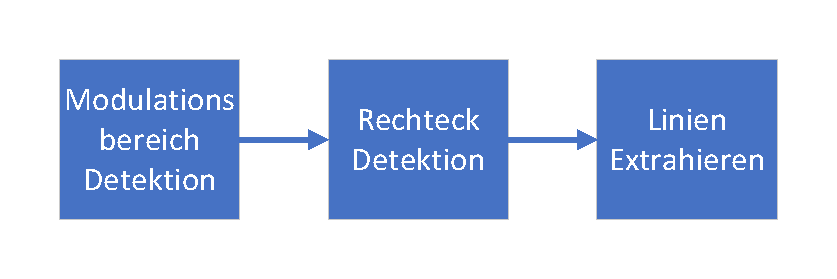
\includegraphics[keepaspectratio,width=1.0\textwidth]{images/4_ZweiteErfahrung/Strukturdiagramm.pdf}
 \caption{Strukturdiagramm}
 \label{fig:Strukturdiagramm für zweite Methode}
\end{figure}


Das Objekt, das mit dieser Methode bearbeitet wird, ist auch ein Reihe von Bildern, die von einer Handkamera aufgenommen wurden. Durch eine Bildregistration Operation diese Bilder in dasselbe Koordinatensystem umgewandelt. Mit gegenseitige Subtraktion erhalten eine Reihe Differenzbildern. Durch das Wissen des vorherigen Kapitels, die $``Energie"$ wird hauptsächlich aus diesem Modulationsbereich gewonnen. Nehmen einige mit maximale $``Energie"$ Differenzbildern addieren und eine detektierendes Bild erhalten, um die folgende Operation zu behandeln. Diese zwei Teilbereiche sind schon in vorherigen Kapitel geschrieben und werden hier nicht ins Detail gehen. Um den Modulationsbereich vom Bild hervorzuheben, nehmen das detektierendes Bild eine Binariesierung Operation, dadurch wird das Bild in zwei Teilen geteilt, eine für Objekt (hier heißt die Modulationsbereich) und eine für Hintergrund (hier heißt die Bereich umgeben die Modulationsbereich). Danach zur Beseitigung der zahlreiche Unvollkommenheiten (hier heißt kleine Punkte und Lücken), die von Rauschen und Fehler verursacht werden, brauchen hier eine morphologische Behandelung, welche basiert von das Form und Struktur des Objekts. Als nächste soll die Modulationsbereich erkannt werden. Um diese zu implementieren, muss die rechteckigen Grenzen zwischen Modulationsbereich und Hintergrundbereich finden. Mit Helfe einer Kantenextraktionsmethode, hier Canny-Algorithmus benutzen, werden im Bild nur die Kanten beleibt, die die Grenze des Modulationsbereich enthält. Beobachten, dass die Grenze des Modulationsbereichs ein rechteckig Form ist, besteht sie aus vier Linien. Das Hough-Transformationsverfahren wird verwendet, um jede zwei gerade Linien in der horizontalen Richtung bzw. der vertikalen Richtung zu erfassen. Schließlich wird das endgültige Rechteck durch die vier geraden Linien bestimmt, das heißt, der Modulationsbereich wird bestimmt. Die Flussdiagramm wird in Abbildung \ref{fig:Flussdiagramm der zweite Methode} gezeigt. Die Details jedes Teils werden in den folgenden Abschnitten beschrieben.

\begin{figure}[H]
 \centering 
 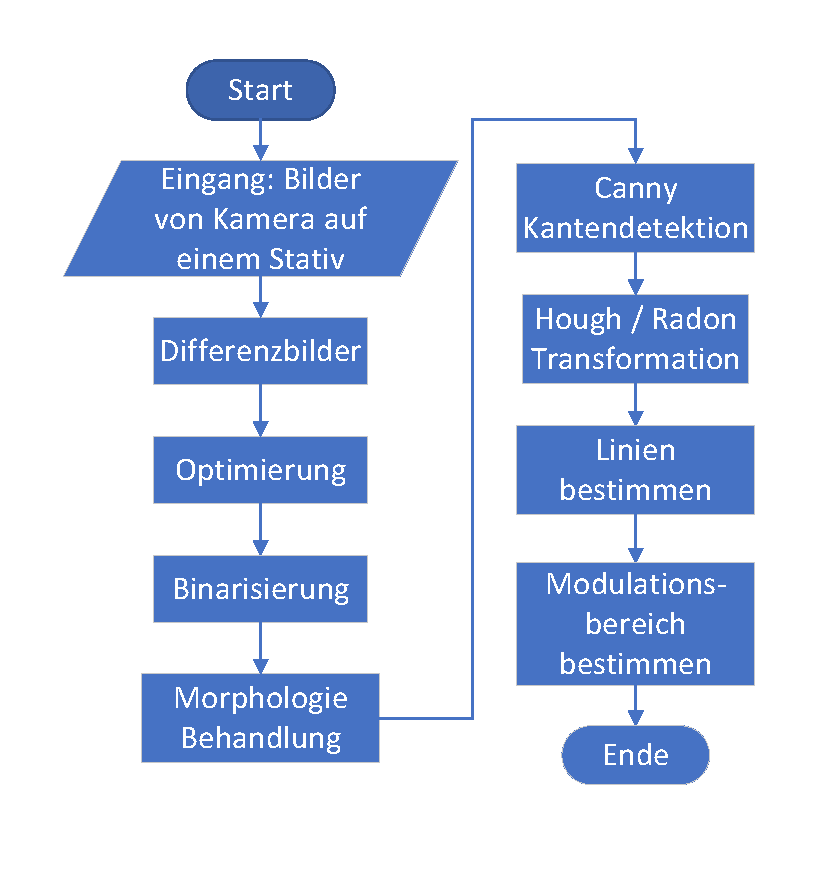
\includegraphics[keepaspectratio,width=1.0\textwidth]{images/4_ZweiteErfahrung/Flussdiagrammsum.pdf}
 \caption{Flussdiagramm der Methode}
 \label{fig:Flussdiagramm der zweite Methode}
\end{figure}

\section{Binarisierung}

In diesem Abschnitt wird der Binarisierungsvorgang der Bildverarbeitung beschrieben. Hier um die Modulationsbereich zu detektieren, muss zuerst es vom Bild hervorzuheben. Dann mit einer Binarisierung Operation kann das implementieren, indem das Bild in zwei Teilen geteilt, ein Teil mit Pixelwert 1 für die Modulationsbereich, anderes mit Pixelwert 0 für die umgebende Hintergrund. Dann kann die Modulationsbereich mit einige weitere Operationen behandelt werden.

In der digitalen Bildverarbeitung nehmen binäre Bilder eine sehr wichtige Position ein. Viele Anwendungen der digitalen Bildverarbeitung können als binäre Probleme betrachtet werden. Um binäre Bilder zu verarbeiten und zu analysieren, digitalisieren zunächst das Graustufenbild, um ein binäres Bild zu erhalten. Wenn das Bild weiterverarbeitet wird, bezieht sich die Sammeleigenschaft des Bildes nur auf die Position des Pixels, dessen Pixelwert 0 oder 255 ist, und der mehrstufige Wert des Pixels ist nicht länger beteiligt, so dass die Verarbeitung einfach ist. Darüber hinaus ist die Menge an Datenverarbeitung und Komprimierung gering. 

Um ein ideales Binärbild zu erhalten, werden im Allgemeinen geschlossene, zusammenhängende Grenzen verwendet, um Bereiche zu definieren, die sich nicht überlappen. Hier geben ein einfaches Beispiel zur Veranschaulichung der Binarisierungsvorgang. Annehmen ein Fall mit einen bimodalan Histogramm des Bildes. Abbildung \ref{fig:Histogramm} zeigt einen solchen Histogramm. Darin gibt es zwei scharfe Wellenberg, eine für das Objekt und eine für den Hintergrund. Die Binarisierungsschwelle T wird genau an die tiefste Stelle zwischen den beiden Wellenberg gelegt. 

\begin{figure}[htb]
 \centering 
  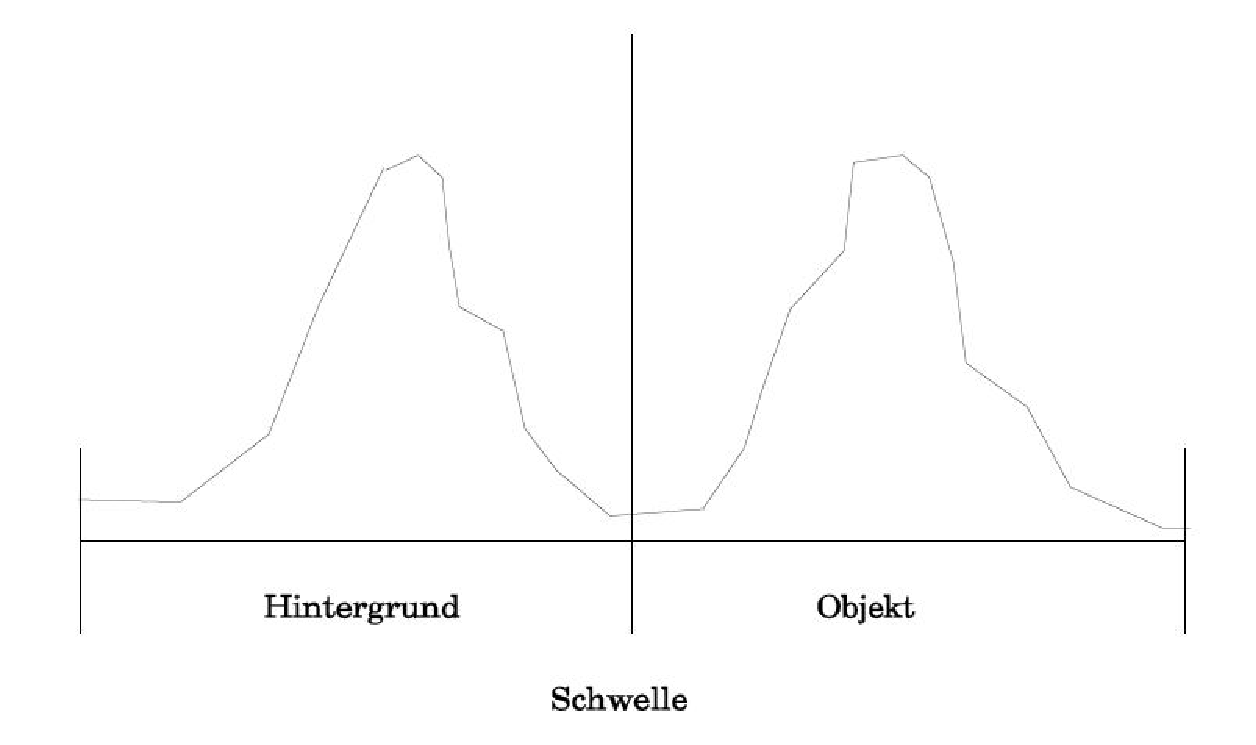
\includegraphics[keepaspectratio,width=0.6\textwidth]{images/4_ZweiteErfahrung/Binar/binar.pdf}
 \caption{Histogramm für einen einfachst Beispiel}
 \label{fig:Histogramm}
\end{figure} 

Alle Pixel, deren Graustufe größer oder gleich dem Schwellenwert T ist, werden als zu einem bestimmten Objekt gehörend bestimmt und ihr Pixelwert ist 1. Andernfalls werden diese Pixel aus dem Objektbereich ausgeschlossen, und der Pixelwert ist 0, was den Hintergrund oder den Ausnahmeobjektbereich anzeigt. Die Formel darstellt als:

\begin{equation}
  y(x) =
  \begin{cases} 
  0,   & \mbox{für }x < T \\
  1, & \mbox{sonst}
  \end{cases}
\end{equation}

In der Praxis ist das Histogramm aufgrund der Helligkeit und Inhalt des Bilds nicht der obige bimodale Fall. Dies erfordert auch, dass die geeignete Binarisierungsmethode entsprechend den tatsächlichen Bedürfnissen im Binarisierungsprozess auswählen. Als folgende werden einige in diese Arbeite versuchte Binarisierungsmethoden vorstellen.

\textbf{Grundlegende globale Schwelle Methode}

Der grundlegende globale Schwelle Methode ist eine Erweiterung des festen Schwelle Methode, die vorher beschriebt. Wenn die Histogrammspitzen und -täler des Bildes offensichtlich sind und Doppelpeaks aufweisen, ist die Wirkung dieser Methode besser. Es basiert auf der visuellen Überprüfung des Histogramms und der Schwellenwert wird durch eine iterative Methode erhalten. Die grundlegende Algorithmus ist wie folgt:

1. Wählen eine Paramenter t und einen anfänglichen Schwellenwert $ T_{0} $ aus, wobei der Durchschnitt der maximalen Grauwerte $ l_{max} $ und minimalen Grauwerte  $ l_{max} $ verwendet wird. $ T_{0} = (l_{max}+l_{max})/2 $

2. Segmentieren das Bild mit dem Schwellenwert $ T_{0} $. Dann das Bild besteht aus zwei Teilen: $ G_{1} $ besteht aus die Pixeln mit deren Grauwert größer als $ T_{0} $ und dargegen $ G_{2} $ deren Grauwert kleiner oder gleich als $ T_{0} $.

3. Berechnen den durchschnittlichen Grauwert aller Pixeln in $ u_{1} $ und $ u_{2} $ und den neue Schwellenwert $ T_{1} = (u_{1}+u_{2})/2 $.

4. Falls $ |T_{0} - T_{1}| < t $, dann nehmen $ T_{1} $ als optimalen Schwellenwert. Andernfalls weisen $ T_{1} $ zu $ T_{0} $und wiederholen die Schritte $ 2\sim4 $, bis der optimale Schwellenwert erhalten ist.

Abbildung. 

\textbf{Grundlegende lokale Schwellenwert Methode}

Ein Bildgebungsfaktor ungleichmäßiger Helligkeit bewirkt, dass ein Histogramm, das ansonsten für eine effiziente Segmentierung geeignet wäre, ein Histogramm wird, das nicht effektiv mit einem einzigen globalen Schwellenwert segmentiert werden kann.

Ein Verfahren zur Verarbeitung besteht darin, das Bild weiter in Unterbilder zu unterteilen, um unterschiedliche Unterbilder mit unterschiedlichen Schwellenwerten zu segmentieren. Diese Methode wird als grundlegende adaptive Schwellenwert-Binarisierungsmethode bezeichnet. Das Hauptproblem bei diesem Ansatz besteht darin, das Bild zu unterteilen und den Schwellenwert für das resultierende Teilbild abzuschätzen. Da die Schwelle für jedes Pixel von dem Pixel in der Untergruppe abhängt, die Position im Bild, also solche Schwellen sind adaptiv. 

Ein Verfahren zum Unterteilen von Unterbildern wird für das Bild übernommen. Hier werden drei Arten von Unterteilungsverfahren ausgewählt, und Unterbildermit einer Größe von $ 32\times32,4 \times4,16\times16 $ Pixelwerden jeweils geteilt, und die durchschnittliche Graustufe der Unterbilder wird Sals ein Schwellenwert für die Binärisierung ausgewählt.

Abbildung. 

\textbf{OTSU adaptive Schwelle Methode}

OTSU\cite{Ostu}, auch bekannt als die maximale Interklassenvarianz, wurde 1979 vom japanischen Gelehrten Otsu vorgeschlagen und ist eine adaptive Schwellenwertbestimmungsmethode, die auch als Otsu bekannt ist.

Die Grundidee des Otsu-Algorithmus ist: Verwenden das Histogramm des Bildes, gemäß der Varianz zwischen dem Vordergrund und dem Hintergrund, um den optimalen Schwellenwert dynamisch zu bestimmen. Setze die Anzahl der Pixeln in einen Bilden ist N, die Graustufe ist $ L(0,1,...,L-1) $. Die Anzahl der Pixeln mit dem Grauswert i ist $ n_{i} $, dann die Wahrscheinlichkeit von i läuft $ P_{i} = \frac{n_{i}}{N} $. Für das Bild stellt das T die Segmentierungsschwellenwert zwischen Vordergrund und des Hintergrund dar. Vordergrund entsprecht die Grauswerte von 0 zu $ T-1 $, dagegen Hintergrund die Grauswerte von T zu $ L -1 $.

Die Wahrscheinlichkeit der Vordergrundgebiet W0 und der durchschnittliche Grauwert U0 sind

\begin{equation}
  w_{0} = \sum_{i=0}^{T-1} p_{i},\quad u_{0} = \sum_{i=0}^{T-1} ip_{i}/w_{0}
\end{equation}

dagegen die Wahrscheinlichkeit der Hintergrundpunkte W1 und der durchschnittliche Grauwert U1 sind

\begin{equation}
  w_{1} = \sum_{i=T}^{L-1} p_{i} = 1-w_{0},\quad u_{1} = \sum_{i=T}^{L-1} ip_{i}/w_{1}
\end{equation}

Dann das gesamte durchschnittliche Grauwert des Bildes ist

\begin{equation}
• u = w_{0}u_{0} + w_{1}u_{1}
\end{equation}

Die Infra-Klassen-Varianz ist definiert als

\begin{equation}
•\sigma^2 = w_{0}(u_{0} - u)^2 + w_{1}(u_{1} - u)^2 = w_{0}w_{1}(u_{0} - u_{1})^2
\end{equation}

Nehmen Schwellenwert T von 0 zu $ L-1 $. Wenn $ sigma^2 $ Maximum ist, wählen der entsprechende T als der optimale Schwellenwert aus.

Die Ostu-Methode verwendet Grauswert Histogramm zur Bestimmen des Schwellenwerts. Es ist eine automatisch non-parametrische Schwellenauswahlmethode. Diese Methode ist einfach zu berechnen, und wird nicht von der Kontrast- und Helligkeitsänderung unter bestimmten Bedingungen beeinflusst und kann das Objekt zufriedenstellend vom Hintergrundbereich trennen.

Abbildung. 















\section{Morphologie}

Nach der Binarisierung kann das Bild zahlreiche Unvollkommenheiten erhalten. Insbesondere ist das Binärbild, die durch einfache Schwellenwert erteilt werden, durch Rauschen und Textur verzerrt. Die morphologische Bildverarbeitung verfolgt das Ziel, diese Unvollkommenheiten zu beseitigen, indem Form und Struktur des Objekts berücksichtigt werden.

Morphologische Operationen arbeiten auf der Grundlage der Mengenoperation und hängen von der relativen Ordnung des Pixelwerts ab. Diese Eigenschaft macht es besonders geeignet für die Verarbeitung von Binärbildern. Natürlich ist Mengenoperation gleichmäßig gültig für Graustufenbilder. Hier in dieser Arbeit wird es nur in binäre Bilder benutzt. Es erstellt ein neues Binärbild, bei dem das Pixel einen nicht-Null Wert hat, nur wenn der Operation an dieser Position im Eingabebild erfolgreich ist.

Die Eingabedaten für die mathematischen morphologischen Operationen sind zwei Bilder: das zu bearbeitende Bild A und ein Strukturelement B. B ist normalerweise eine kleine Pixelmatrix mit jeweils einem Wert von Null oder Eins. Einige Eigenschaft des Strukturelements werden wie folgend gelegt.

\begin{itemize}

\item Die Matrixdimensionen geben die Größe des Strukturelements an.
\item Das Muster, das aus Einsen und Nullen bestehen, gibt die Form des Strukturelements an.
\item Ein Ursprung des Strukturelements ist üblicherweise eines dessen Pixel, es verlassen sich auch außerhalb des Strukturelements liegen. 

\end{itemize}

Eine übliche Praxis besteht darin, dass ungerade Dimensionen der Pixelmatrix stellen und den Ursprung als das Zentrum der Matrix definieren. Einige grundlegende Strukturelement legt als folgen:

\begin{figure}[htb]
 \centering 
  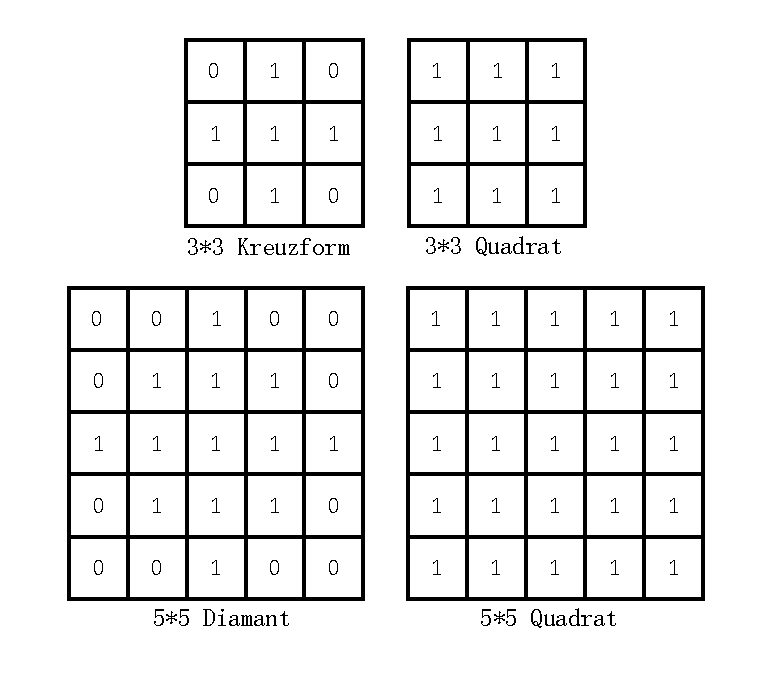
\includegraphics[keepaspectratio,width=0.6\textwidth]{images/4_ZweiteErfahrung/Morphological/strelement.pdf}
 \caption{Einige grundlegende Strukturelement}
 \label{fig:Strukturelement}
\end{figure} 

Als folgend werden zuerst die zwei grundlegende morphologischen Operatoren Erosion und Dilatation beschrieben. Anschließen vorstellen die darauf basierend Operationen, wie als Öffnung und Schließung bekannt sind.

\textbf{Dilatation}

Die Dilatation Operation bewirkt, dass das Objekt nach größer wächst. Das wächst Ausmaß hängt von der Art und Form des Strukturelements ab. Die Formel eine Dilatation wird darstellt als:

\begin{equation}
•A \oplus B =\lbrace z \mid \widehat{(B)_z} \cap A \ne \varnothing \rbrace  
\end{equation}

Hier $ \widehat{(B)_z} $ heißt Strukturelement B um seinen Ursprung reflektiert und um z verschoben. Die entsprechende Dilatation für das Bild A mit B ist die Menge aller Verschiebungen z, die $ \widehat{B} $ und A mindestens ein gemeinsames Element habe. Das Ergebnis der Dilatation läuft, die Pixeln um den Grenze des Objekts hinzufügen. Außerdem die Dilatation Operation wird im wesentlichen verwendet um die Löcher (fehlende Pixel) in einem kontinuierlichen Objekt zu füllen. Es beeinflusst die Intensität an diesem Bereich und kann als ein Unschärfe Effekt beobachtet werden, nämlich eine räumlichen Tiefpassfilter, die beim linearen Filtern des Bildes verwendet werden. Abbildung \ref{fig:Dilatation und Erosion} zeigt eine typische Dilatation Operation.

\begin{figure}[htb]
 \centering 
  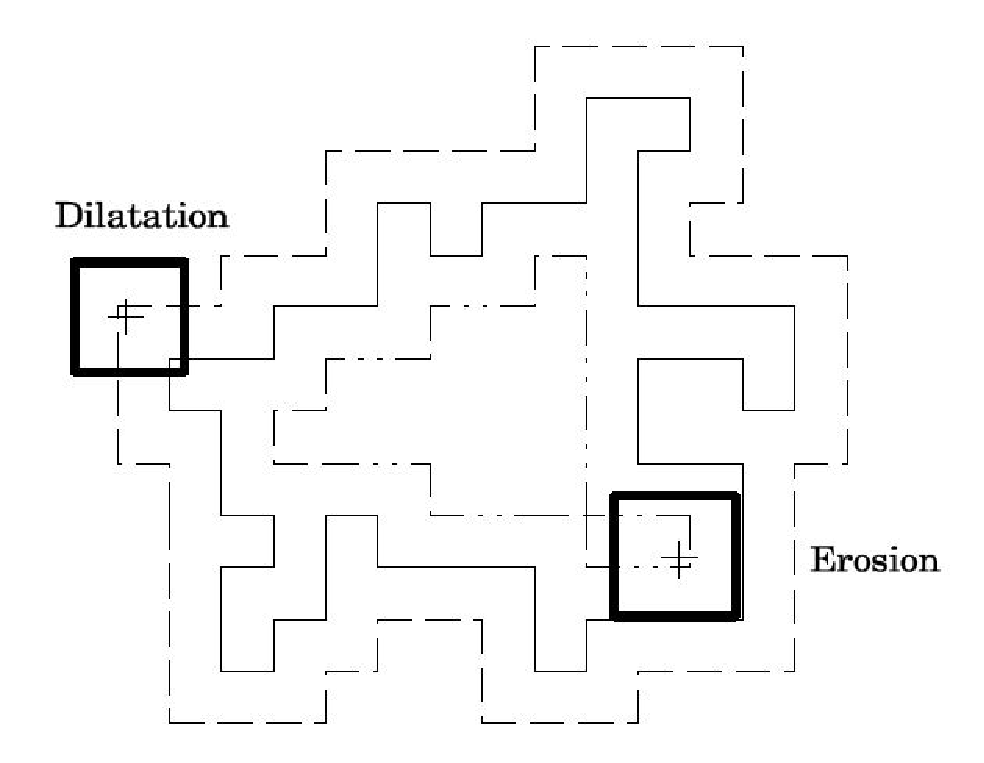
\includegraphics[keepaspectratio,width=0.8\textwidth]{images/4_ZweiteErfahrung/Morphological/DilatationundErosion.pdf}
 \caption{Dilatation und Erosion}
 \label{fig:Dilatation und Erosion}
\end{figure} 


\textbf{Erosion}

Der Operationseffekt eine Erosion ist genau ein Gegenteil von Dilatation. Die Erosion Operation bewirkt, dass das Objekt nach kleiner wechseln. Die Erosion eines Bildes A durch das Strukturelement B ist definiert als 

\begin{equation}
•A \ominus B =\lbrace z \mid (B)_z \subseteq A \rbrace  
\end{equation}

Hier die Erosion des Bilds A ist die Menge aller Punkte z mit derart, dass das Strukturelement B von verschieben wird, zu eine Teilmenge des Bildes A 	gehört. Diese Operation führt zu einem Verlust von Grenzpixeln des Objekts.

Die Erosion Operation entfernt solche Strukturen, die eine kleinere Größe als das strukturierende Element haben. Dann kann es verwenden wird, um die verrauschte "Verbindung" zwischen zwei Objekten zu entfernen. Da die unerwünschten Pixel entfernen werden, ist der Effekt als ein Schärfen des Objekts entsprechen. Als folgend in Abbildung \ref{fig:Dilatation und Erosion} zeigt eine typische Erosion Operation.


\textbf{Öffnung}

Die Öffnung Operation eines Bildes ist eine kombinatorische Operation von Erosion und Dilatation, d.h. zuerst nehmen eine Erosion Operation, danach eine Dilatation Operation. Praktisch werden Bild A durch beide Operationen mit dem gleichen Strukturelement B ausgeführt. Die Formel einer Öffnung Operation ist definiert als

\begin{equation}
•A \circ B =( A \ominus B )\oplus B  
\end{equation}

Die Grenze des geöffneten Objekts sind die Punkte, dass Strukturelement B die äußersten Punkte der Grenze von Objekt erreicht, wenn B innerhalb dieser Grenze entlangfahren. Feine strukturierte Details,
kleiner als das Strukturelement werden demnach beim Öffnung Operation entfernt, dünne Verbindungen zwischen größeren Teilen aufgelöst. Eine Öffnung Operation wird in Abbildung \ref{fig:oeffnungundschliessung} gezeigt.

\begin{figure}[htb]
 \centering 
  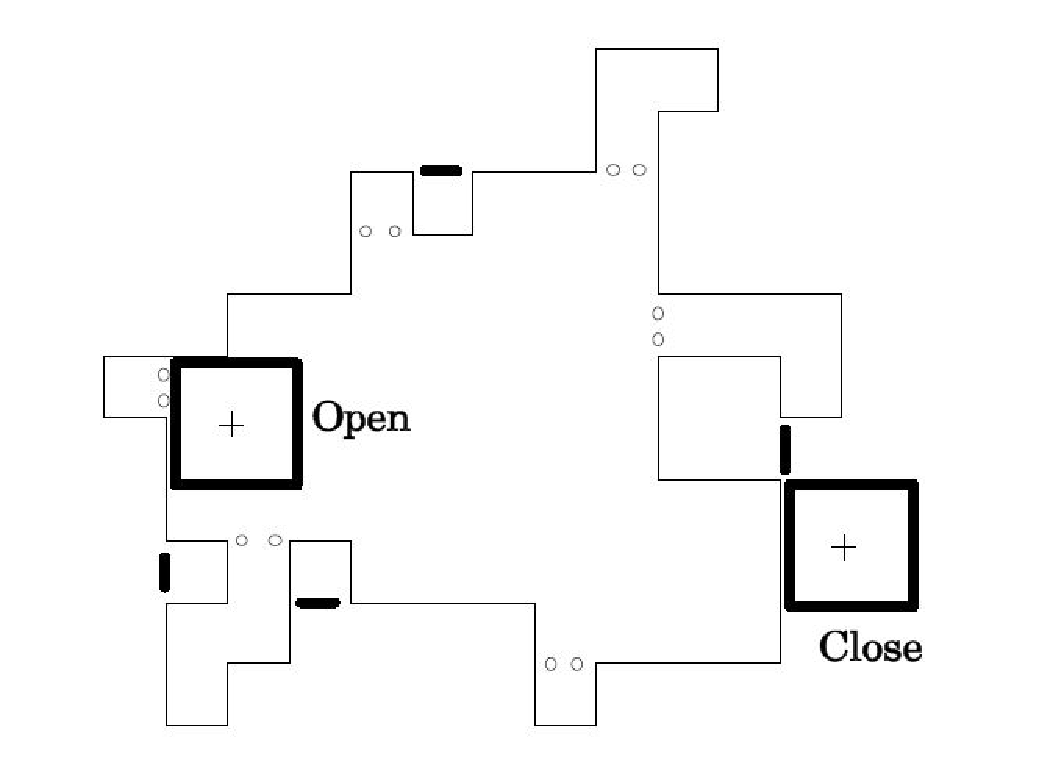
\includegraphics[keepaspectratio,width=0.8\textwidth]{images/4_ZweiteErfahrung/Morphological/oeffnungundschliessung.pdf}
 \caption{Einige grundlegende Strukturelement}
 \label{fig:oeffnungundschliessung}
\end{figure} 

\textbf{Schließung}

Gleichfalls mit Öffnung Operation ist die Schließung Operation auch eine kombinatorische Operation von Erosion und Dilatation. Der Unterschied dazwischen legt der Reihenfolge der Operation, d.h. hier zuerst eine Dilatation Operation, danach eine Erosion Operation mit dem gleichen Strukturelement. Das Schließung eines Bildes A durch das Strukturelement B ist definiert als

\begin{equation}
•A \bullet B =( A \oplus B )\ominus B  
\end{equation}

Die Grenze des geschlossenen Objekts sind die Punkte, dass Strukturelement B, die die äußersten Punkte der Grenze von Objekt erreichen, wenn B außerhalb dieser Grenze entlangfahren. Kleinere Risse, Lücken und feine Details werden dagegen aufgefüllt und mit den großen Teilen zusammengeschlossen. Abbildung \ref{fig:oeffnungundschliessung} zeigt eine Vorgang der Schließung Operation.


Öffnung und Schließung Operation besitzen die folgenden Eigenschaften:

\begin{itemize}

\item Öffnung und Schließung sind idempotent.
\item Die Öffnung Operation ist anti-extensiv. 
\item Die Schließung Operation ist extensiv.
\item Öffnung und Schließung sind dual bezüglich der Komplementierung.
\item Bezeichnet ein Bild als B-Öffnet, wenn es bezüglich gleicher Öffnung Operation unverändert bleibt. 
\item Bezeichnet ein Bild als B-Schließt, wenn es bezüglich gleicher Schließung Operation unverändert bleibt. 

\end{itemize}


\section{Canny detection}

Jetzt können wir ein Binärbild erhalten, das grob in zwei Teile geteilt werden kann, einen Modulationsbereich mit Pixelwert 1 im mittleren und einen umgibt Hintergrundbereich mit Pixelwert 0. Um die nächste Linie Detektion zu implementieren. Machen eine Kanten Detektion, weil Kanten oft mit den Grenzen von Objekten in einer Szene verknüpft werden. Hier ist es die Grenze zwischen Modulationsbereich und Hintergrundbereich. \cite{canny}

Es gibt immer einige gut Kantenextraktionmethod, wie Sobel, Canny, Laplacian, Prewitt, Roberts usw. Hier in dieser Abreit wird die leistungsfähigste Kantenerkennungsmethode bzw. Canny Algorithmus benutzt. Die Canny-Methode unterscheidet sich von den anderen Kantenerkennungsmethoden darin, dass sie zwei verschiedene Schwellenwerte verwendet (um starke und schwache Kanten zu erkennen) und die schwachen Kanten in der Ausgabe nur dann einschließt, wenn sie mit starken Kanten verbunden sind. Diese Methode kann daher im Vergleich zur anderen Method weniger Wahrscheinlichkeit verfügen, durch Rauschen getäuscht zu werden, und mehre Wahrscheinlichkeit verfügen, echte schwache Kanten zu erkennen.

Das Ziel von Canny Algorithmus ist es, einen optimalen Kantenextraktionsalgorithmus zu finden. Drei Kriterien für die optimale Kantendetektion werden vorgeschlagen:

\begin{itemize}

\item Gute Erkennung: Der Algorithmus kann so viele tatsächliche Kanten wie möglich im Bild erkennen.
\item Gute Positionierung: Identifizieren die Kanten so nah wie möglich an den tatsächlichen Kanten im Bild.
\item Minimale Antwort: Kanten in einem Bild können nur einmal identifiziert werden, und mögliches Bildrauschen sollte nicht als Kanten erkannt werden.

\end{itemize}

Die Implemetierung eine Canny Algorithmus läuft:

\begin{enumerate}
	\item \textbf{Gaußsche Unschärfe.} Die Hauptziel ist, Rausch zu entfernen. Da die Rauschen auch auf Hochfrequenzsignale konzentriert ist, wird es leicht als eine falsche Kante erkannt. Anwenden gaußsche Unschärfe, um Rauschen zu entfernen und die Erkennung falscher Kanten zu reduzieren. Es sollte beachtet werden, dass ein zu großer Radius einige schwache Kanten nicht erkennen.
	\item \textbf{Berechnen die Größe und Richtung des Gradienten.} Die Kanten des Bildes können in verschiedene Richtungen zeigen. Daher verwendet der klassische Canny Algorithmus vier Gradientenoperatoren, um die Gradienten in horizontaler, vertikaler und diagonaler Richtung zu berechnen. Jedoch in allgemeine werden diese vier Gradientenoperatoren nicht verwendet, sondern mit Kantenunterschiedsoperatoren (wie Rober, Prewitt, Sobel) die Differenz Gx und Gy in horizontaler und vertikaler Richtung berechnen. Die Berechnung der Gradientengröße und Richtung wie folgt:	
\begin{equation}
\begin{split}
•  G   & = \sqrt{G_x^{2} + G_y^{2}} \\
\theta & = atan2(G_y,G_x)
\end{split}
\end{equation}

Der Gradientenwinkel $ \theta $ liegt im Bereich von Radianten $ -\pi $ bis $ \pi $, dann approximiere es in vier Richtungen, die horizontale, vertikale und zwei diagonale Richtungen repräsentieren    $(0^{\circ}, 45^{\circ}, 90^{\circ}, 135^{\circ}) $. Es kann durch $  \pm i \pi / 8\ (i =1, 3, 5, 7) $ geteilt werden, und der in jedem Bereich fallende Gradientenwinkel einen spezifischen Wert ergibt, der eine von vier Richtungen repräsentieren. Als folgend nehmen eine Beispile mit Sobel Operator.

\begin{equation}
G_x = \begin{bmatrix}
-1 &0 &+1 \\
-2 &0 &+2 \\
-1 &0 &+1
\end{bmatrix} * A \quad and \quad G_y = \begin{bmatrix}
+1 &+2 &+1 \\
0 &0 &0 \\
-1 &-2 &-1
\end{bmatrix} * A
\end{equation}
	
	\item \textbf{Nicht-maximale Unterdrückung.} Nicht-maximale Unterdrückung ist eine Kantenverfeinerungsmethode. Die Gradientenkanten, die normalerweise abgeleitet werden, sind nicht als ein Pixel breit, sonder mehrere Pixel breit. Während Kriterie 3 erfordert, dass die Kante nur eine genaue Punktbreite hat. Nicht-maximale Unterdrückung kann dazu beitragen, den lokalen maximalen Gradienten beizubehalten, während alle anderen Gradientenwerte unterdrückt werden. Dies bedeutet, dass nur die schärfste Position in der Gradientenänderung beibehalten wird. Der Algorithmus ist wie folgt:
	\begin{itemize}
	\item Vergleichen die Gradientenstärke des aktuellen Punkts mit der Gradientenstärke der positiven und negativen Gradientenrichtungspunkte.
	\item Wenn die Gradientenstärke des aktuellen Punktes im Vergleich zur Gradientenstärke anderer Punkte in der gleichen Richtung am größten ist, wird der Wert auf 1 behalten. Ansonsten wird es auf 0 gesetzt. Zum Beispiel, wenn die Gradientenrichtung des aktuellen Punktes in die Richtung von $(90^{\circ}$ direkt darüber zeigt, muss es mit den Pixeln in der vertikalen Richtung direkt darüber und darunter verglichen werden.
	\end{itemize}
	
	Es ist erwähnenswert, dass die positiven und negativen Richtungen keine unterschiedlichen Bedeutungen haben. Zum Beispiel sind die südöstliche Richtung und die nordwestliche Richtung beide als eine Richtung der Diagonalen betrachtet. Vorher approximierten die Gradientenrichtung horizontal, vertikal und zwei Diagonalen in vier Richtungen, so dass jedes Pixel in einer dieser vier Richtungen entsprechend seiner eigenen Gradientenrichtung verglichen wird, um zu bestimmen, ob es beibehalten wird. 
	
	
	\item \textbf{Doppelte Schwelle.} Ein allgemeiner Kantenerkennungsalgorithmus verwendet einen Schwellenwert, um kleine Gradientenwerte entfernen, die durch Rauschen oder Farbänderungen verursacht werden, während große Gradientenwerte beibehalten werden.
Der Canny Algorithmus wendet einen doppelten Schwellenwert, d.h. einen hohen Schwellenwert und einen niedrigen Schwellenwert an, um Kantenpixel zu unterscheiden. Wenn der Kantenpixelpunktgradientwert größer als den hohen Schwellenwert ist, wird er als einen starken Kantenpunkt betrachtet.	Wenn der Kantengradientenwert kleiner als der hohen Schwellenwert und größer als den niedrigen Schwellenwert ist, wird er als einen schwachen Kantenpunkt markiert. Punkte, die unterhalb der niedrigen Schwelle, werden unterdrückt.

	\item \textbf{Hysterese Grenzenverfolgung.} Bisher können die starke Kantenpunkt als echte Kanten angesehen werden. Dagegen die Schwache Kantenpunkte können echte Kanten sein, jedoch sie können auch durch Rauschen oder Farbänderungen verursacht sein. Um genaue Ergebnisse zu erhalten, sollten die zweite Möglichkeit von schwachen Kantenpunkte entfernt werden. In allgemein werden die schwache Kantenpunkte und die starke Kantenpunkte, die durch reale Kanten verursacht werden, als verbunden betrachtet, während die schwache durch Rauschen verursacht Kantenpunkte, dies nicht verbunden sind. Der sogenannte Hysterese Grenzenverfolgung Algorithmus untersucht die achte verbundene Pixel eines schwachen Kantenpunktes, solange ein starker Randpunkt vorhanden ist, wird dieser schwache Randpunkt als echt Kantenpunkte betrachtet und die Wert als 1 bleibt.
	
Zur Implementierung dieser Schritt sucht allen verbundenen schwachen Kanten. Wenn ein Punkt einer verbundenen schwachen Kante mit einem starken Kantenpunkt verbunden ist, wird die schwache Kante beibehalten, snsonsten unterdrücken diese schwache Kante. Bei der Suche kann der Algorithmus "Breite zuerst" oder "Tiefe zuerst" verwenden. Nachdem der gesamten Suche des Bildes, werden die Nicht-Kantenpunkte entfernt, d.h. der Wert auf 0 gesetzt wird.
	
\end{enumerate}

Abbildung \ref{fig:canny} zeigt ein Ergibnis mit Canny Kantenextraktion.

\begin{figure}[H]
 \centering 
  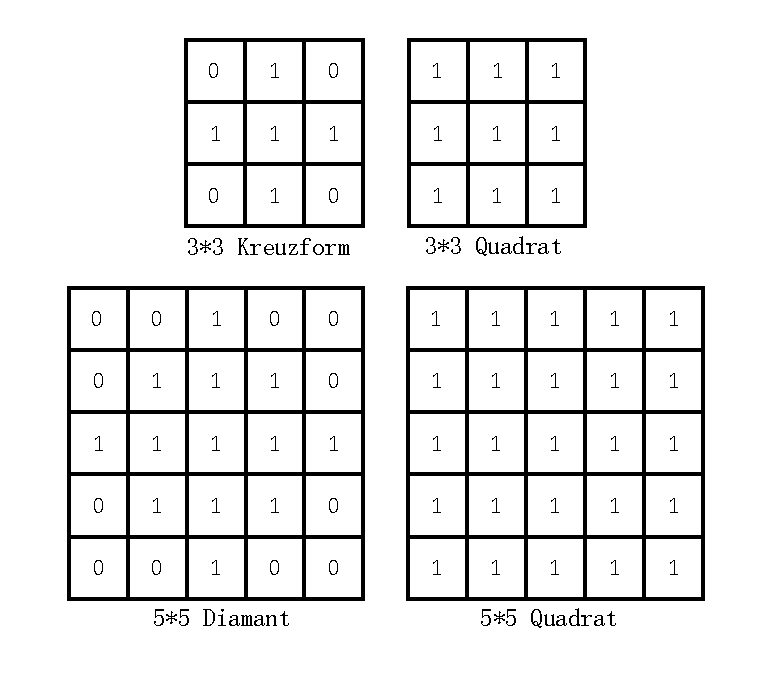
\includegraphics[keepaspectratio,width=0.4\textwidth]{images/4_ZweiteErfahrung/Canny/canny.pdf}
 \caption{Einige grundlegende Strukturelement}
 \label{fig:canny}
\end{figure} 

\section{Hough Transformation}

Hier betrachten die Grenzen des modulierten Rechtecks als Linien. Dann das Problem für Rechteck Detektion umwandeln nach das Problem eines Linie Extrahieren. Um dies zu tun, müssen die Kanten erkennen, die auf einer geraden Linie durch das Bild liegen. Die Hough Transformation ist eine beliebte Methode zum Extrahieren von Linien aus einem Bild. Es kann solche Informationen liefern, indem die Spitzen an Punkten die geraden Linien in dem binären Bild entsprechen. Der Aufwand für eine Hough Transformation hängt von der Größe des Bildes und der Anzahl der analysierten Winkel ab. Da die Winkelauflösung für die weitere Verarbeitung wichtig ist, ist eine maximale Kameraneigung vorgeschrieben. Hier in diese Arbeit läuft es $ \pm 10^{\circ} $.


Um die Funktionsweise des HT Algorithmus zu beschreiben, müssen einige Definition einfügen. In Hough Transformation, jede Linie in der $ xy $ Ebene kann parametrisch beschreiben als:
\begin{equation}
•  \rho = x \cos \theta + y \sin \theta
\end{equation} 

Hier bedeutet $ \rho $ die Entfernung vom Ursprung der Koordinate zur Linie, $ \theta $ der Winkel zwischen $ \rho $ und der positiven Richtung der x-Achse, $ (x,y) $ sind die Punkte auf der geraden Linie, wie in Abbildung \ref{fig:Hough} zeigt.

\begin{figure}[H]
 \centering 
  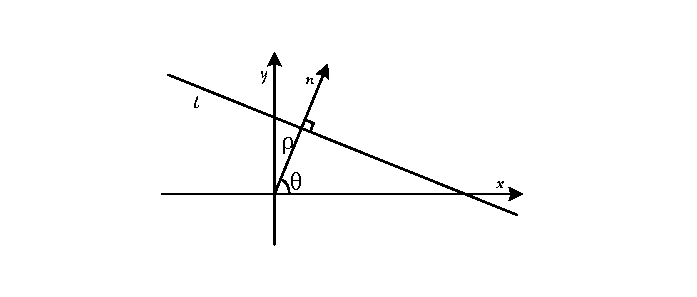
\includegraphics[keepaspectratio,width=1.0\textwidth]{images/4_ZweiteErfahrung/Hough/Hough.pdf}
 \caption{Anglekoordinate}
 \label{fig:Hough}
\end{figure}

Die obige Gleichung gilt für jedes Pixel auf dem Bild, d.h. für jeden Punkt auf dem Bild kann eine entsprechende trigonometrische Kurve nach der Hough-Transformation im Parameterraum ($ \theta $, $ \rho $) gefunden werden. Irgendwelche zwei Punkte auf dem Bild, die zwei  trigonometrische Kurven entsprechen, und werden unvermeidlich einen Schnittpunkt ($ \theta_0 $, $ \rho_0 $) erzeugen. Dieser Schnittpunkt wird dann in die Gleichung der Linie eingefügt, um eine gerade Linie zu bestimmen (nämlich die durch die zwei Punkte auf dem Bild festgelegte Linie). 

Das heißt, die entsprechende trigonometrische Kurven, die von Punkten auf derselben Linie auf dem Bild erzeugt werden, schneiden sich an einem Punkt ($ \theta_0 $, $ \rho_0 $) im Parameterraum. Je mehr Punkte auf der Linie sind, desto mehr Kurven schneiden sich an diesem Punkt. Das Algorithmus einer Hough Transformation wie folgend darstellt:

\begin{enumerate}
\item Erstellen einen Parameterraum mit einer geeigneten Quantisierungsstufe für Entfernung $ \rho $ und Winkel $ \theta $.
\item Erstellen ein Akkumulator Array A($ \rho $,$ \theta $).
\item Erstellen A($ \rho $,$ \theta $) = 0 ,für aller ($ \rho $,$ \theta $).
\item Für jeden Nicht-Hintergrundpunkt $ (x,y) $ im Bild berechnen $ \rho $ mit jede $ \theta $ ,ob Gleichung erfüllen: $ \rho = x \cos \theta + y \sin \theta $. Falls bestimmt, Erhöhe das Akkumulator-Array: $ A(\rho,\theta) = A(\rho,\theta) + 1 $.
\item Suchen den Spitzenwert in Array A, der die Linie im Parameterraum angeben.
\end{enumerate}

Eine Beispiel Implementierung der Hough Transformation zeigt in Abbildung .





